


 
\documentclass[10pt,a4paper,twoside]{article}

\usepackage{PanAfriConAI22}
\usepackage{listings}
\usepackage{graphicx}
\usepackage{float}
\usepackage{color}

\definecolor{bggray}{rgb}{0.25, 0.25, 0.25}




\usepackage{filecontents}
\begin{filecontents}{bibliography.bib}
@misc{shi2016realtime,
      title={Real-Time Single Image and Video Super-Resolution Using an Efficient Sub-Pixel Convolutional Neural Network}, 
      author={Wenzhe Shi and Jose Caballero and Ferenc Huszár and Johannes Totz and Andrew P. Aitken and Rob Bishop and Daniel Rueckert and Zehan Wang},
      year={2016},
      eprint={1609.05158},
      archivePrefix={arXiv},
      primaryClass={cs.CV}
}

@article{DBLP:journals/corr/abs-2107-03312,
  author    = {Neil Zeghidour and
               Alejandro Luebs and
               Ahmed Omran and
               Jan Skoglund and
               Marco Tagliasacchi},
  title     = {SoundStream: An End-to-End Neural Audio Codec},
  journal   = {CoRR},
  volume    = {abs/2107.03312},
  year      = {2021},
  url       = {https://arxiv.org/abs/2107.03312},
  eprinttype = {arXiv},
  eprint    = {2107.03312},
  timestamp = {Tue, 20 Jul 2021 15:08:33 +0200},
  biburl    = {https://dblp.org/rec/journals/corr/abs-2107-03312.bib},
  bibsource = {dblp computer science bibliography, https://dblp.org}
}

@misc{kuleshov2017audio,
      title={Audio Super Resolution using Neural Networks}, 
      author={Volodymyr Kuleshov and S. Zayd Enam and Stefano Ermon},
      year={2017},
      eprint={1708.00853},
      archivePrefix={arXiv},
      primaryClass={cs.SD}
}

@misc{zeghidour2021soundstream,
      title={SoundStream: An End-to-End Neural Audio Codec}, 
      author={Neil Zeghidour and Alejandro Luebs and Ahmed Omran and Jan Skoglund and Marco Tagliasacchi},
      year={2021},
      eprint={2107.03312},
      archivePrefix={arXiv},
      primaryClass={cs.SD}
}

@Article{Nanni2020,
    author={Nanni, Loris
    and Costa, Yandre M. G.
    and Aguiar, Rafael L.
    and Mangolin, Rafael B.
    and Brahnam, Sheryl
    and Silla, Carlos N.},
    title={Ensemble of convolutional neural networks to improve animal audio classification},
    journal={EURASIP Journal on Audio, Speech, and Music Processing},
    year={2020},
    month={May},
    day={26},
    volume={2020},
    number={1},
    pages={8},
    abstract={In this work, we present an ensemble for automated audio classification that fuses different types of features extracted from audio files. These features are evaluated, compared, and fused with the goal of producing better classification accuracy than other state-of-the-art approaches without ad hoc parameter optimization. We present an ensemble of classifiers that performs competitively on different types of animal audio datasets using the same set of classifiers and parameter settings. To produce this general-purpose ensemble, we ran a large number of experiments that fine-tuned pretrained convolutional neural networks (CNNs) for different audio classification tasks (bird, bat, and whale audio datasets). Six different CNNs were tested, compared, and combined. Moreover, a further CNN, trained from scratch, was tested and combined with the fine-tuned CNNs. To the best of our knowledge, this is the largest study on CNNs in animal audio classification. Our results show that several CNNs can be fine-tuned and fused for robust and generalizable audio classification. Finally, the ensemble of CNNs is combined with handcrafted texture descriptors obtained from spectrograms for further improvement of performance. The MATLAB code used in our experiments will be provided to other researchers for future comparisons at https://github.com/LorisNanni.},
    issn={1687-4722},
    doi={10.1186/s13636-020-00175-3},
    url={https://doi.org/10.1186/s13636-020-00175-3}
}

@article{article,
    author = {Yaroslavsky, Leonid},
    year = {2002},
    month = {05},
    pages = {},
    title = {Fast signal sinc-interpolation methods for signal and image resampling}
}

@misc{google_ai_blog_2021, 
    title={Lyra: A new very low-bitrate codec for speech compression}, url={https://ai.googleblog.com/2021/02/lyra-new-very-low-bitrate-codec-for.html}, 
    journal={Google AI Blog}, 
    year={2021}, 
    month={02}
} 

\end{filecontents}

\usepackage[style=authoryear,backend=bibtex]{biblatex}

\addbibresource{bibliography.bib}






% abstract
% introduction + summarize the problem boteler 2019 solves
% challenges faced by computer-based simulations
% results: accuracy in this vs paper
% conclusion
% improvements/optimizations
% bibliography




%-----------------------------------------------------------------------------%
%                          Author, Date and Title Data                        %
%-----------------------------------------------------------------------------%

\renewcommand{\doctitle}        {Modeling Geomagnetic Induced Currents Using Computer-Based Simulations}
\renewcommand{\docheader}       { } 

\renewcommand{\docaffiliation} { }
\renewcommand{\docauthor} { }


% https://www.swpc.noaa.gov/phenomena/coronal-mass-ejections
% https://www.naes.com/news/what-is-a-geomagnetic-disturbance-and-how-can-it-affect-the-power-grid/

%-----------------------------------------------------------------------------%

\begin{document}


% \selectlanguage{english}


%-----------------------------------------------------------------------------%
%                              Title & Author                                 %
%-----------------------------------------------------------------------------%

\title{\doctitle}{\docauthor}{\docaffiliation}

%-----------------------------------------------------------------------------%
%                            Abstract & Keywords                              %
%-----------------------------------------------------------------------------%

\setlength\columnsep{1cm}

\begin{multicols}{2}
		
	{\parindent 3ex 
		\textbf{\textsf{Abstract}} %---\lipsum[1]
		\\
		Geomagnetic disturbances (GMDs) are caused when the sun emits a coronal mass ejection (CME), a large expulsion of magnetic fields. When the CME collides with Earth's magnetic field, the collision generates currents that create Geomagnetically Induced Currents (GICs). GICs can disturb electrical systems in the affected areas. The March 1989 Quebec incident displays an example of the effects of GMDs, causing a nine-hour power outage. \cite{8859181} works to derive the equations necessary to model GMDs. However, computer-based implementations require specific methods for accurate modeling. This project researches the development of a GMD model on a computer using the Julia programming language. 
				
				
		\textbf{\textsf{Keywords:}} Geomagnetic Disturbances, Geomagnetic Induced Currents, Julia}
		
		
	%-----------------------------------------------------------------------------%
	%                                 Section 1                                   %
	%-----------------------------------------------------------------------------%
		
	\section{Introduction}
	%\label{sec:intro}
	Geomagnetic disturbances, also referred to as "geomagnetic storms", are caused by a transfer of energy of charged particles from the sun to the space surrounding Earth. GMDs are especially dangerous due to the variability of their effects. While the presence of GMDs can be predicted, the effect and magnitude cannot be. The currents produced by the GMDs create electric fields at the Earth's surface. The currents can flow into conducting networks such as power grids or telephone networks, damaging equipment and devices in these networks. Based on the scale of the GMD, the effect can be as large as city-wide blackouts. The process to help mitigate the effects of GMDs is made up of three parts. First, data must be collected for the required area. Second, the collected data must be processed by a transfer function model. Lastly, the data from the model can be used to determine the necessary currents to properly power the affected networks. This paper focuses on the implementation of the second stage, the transfer function model. For the model, the 5 layer Quebec model developed in \cite{8859181} is used.
		
		
		
	%-----------------------------------------------------------------------------%
		
	\section{Implementation}
	%\label{ssec:labelxx}
	The implementation of the 5 layer Quebec model is done in the Julia programming language, using \verb|Trapz| for trapezoidal integration, \verb|PyPlot| for plots, and \verb|FFTW| for Fourier transforms. 
	\subsection{Synthetic Dataset}
	First, a synthetic dataset was created for testing. The synthetic field variation was calculated using the sum of 7 sinusoidal functions. The code for the data was implemented using the following code:
	\begin{lstlisting}
A =   [200, 90, 30, 17, 8, 3.5, 1]
Phi = [10, 20, 30, 40, 50, 60, 70]

f = [0.00009259, 0.00020833, 
0.00047619, 0.00111111, 0.00238095, 
0.00555555, 0.025]

function B(t) # Equation (20)
  y = 0
  for i in 1:7
    y += A[i] * sin(
      2 * pi * f[i] * t 
	  + (pi / 180 * Phi[i])
	)
	end
  return y
end

	\end{lstlisting}
		
	Using the \verb|B| function, the synthetic variation can be found for any second \verb|t|. In Julia, this can be implemented simply using the vectorization operators like so:
	\begin{lstlisting}
timestep = 1
X = 1:timestep:86400
Y = B.(X)
	\end{lstlisting}
		
	\begin{figure*}[b!]
		\begin{center}
		    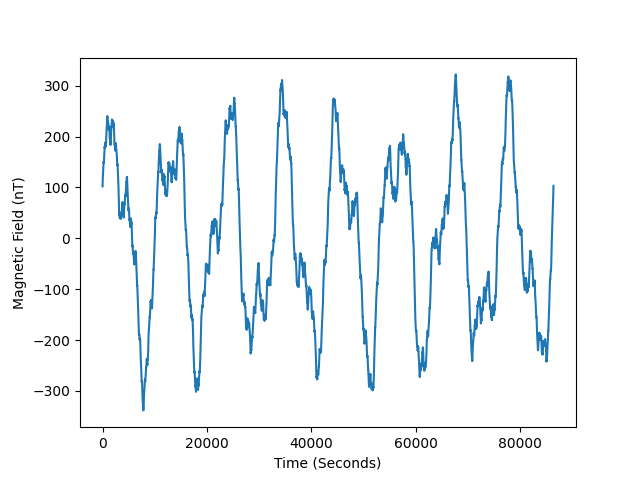
\includegraphics[width=\columnwidth]{Latex/Figure_1.png}
		    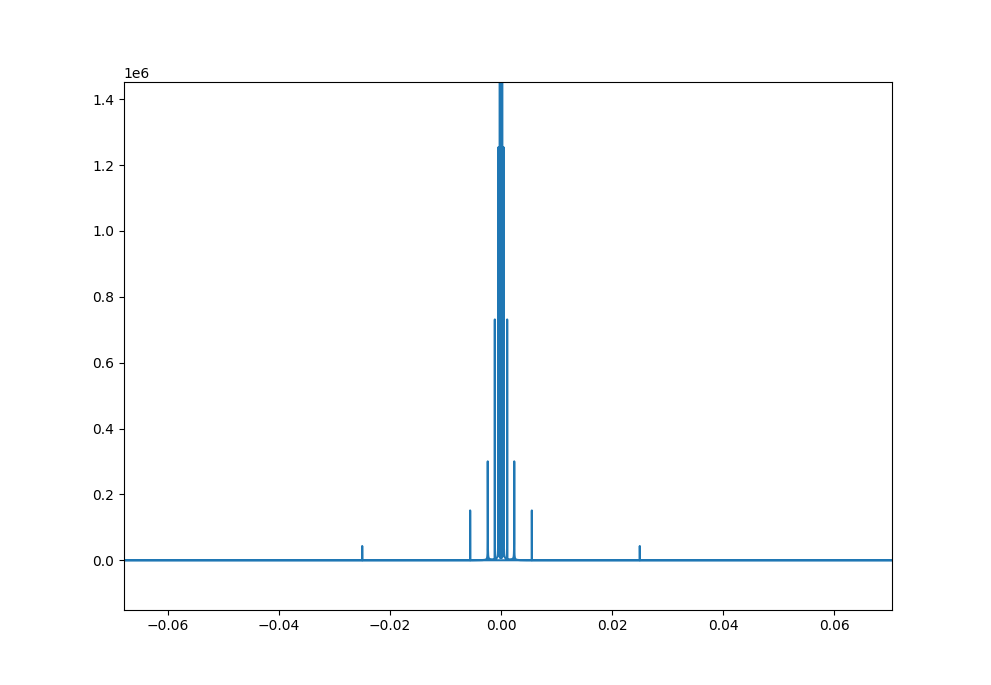
\includegraphics[width=\columnwidth]{Latex/Figure_2.png}
		\end{center}

		\caption{Synthetic Field Variation Graph}
		\caption{Discrete Fourier Transformer of B(t) - A correct implementation should include 7 lines on each side of x=0, representing the 7 sine functions in B(t)}
	\end{figure*}
		
		
	\subsection{Discretization}
	\label{discretization}
	
	Because this implementation is done on a computer with a finite amount of memory, processing power, etc., the continuous function cannot be represented on a computer and must be discretized using a Fourier transform. The following code is used to discretize the \verb|B| function using the FFTW library:
	\begin{lstlisting}
f = fft(Y)
	\end{lstlisting}

    
    Additionally, the horizontal geoelectric field, E(f) is calculated as the convolution of B and K, defined in Julia like so:
    
    \begin{lstlisting}
function K(f)
    mu = pi * 4e-6
    sigma = 1000
    i = 1im
    return sqrt(
        (i * 2 * pi * f) /
        (mu * sigma)
    )
end
    \end{lstlisting}
    
    and the convolution of the signals is calculated like so:
    
    \begin{lstlisting}
freq = fftfreq(length(Y), timestep)
conv = K.(freq) .* f
    \end{lstlisting}
    
    This code creates and processes the synthetic field variation data. Next, a model needs to be developed to model the input data.
    
    
    \subsection{5 Layer Quebec Model}
    The model used in this paper is the 5 layer Quebec model used to model Earth conductivity in \cite{8859181}. The model is represented by 5 equations, each of which use the previous equation. This is implemented in Julia using recursion with the base case being the topmost layer. Each layer has distinct thicknesses and relativities. The thicknesses and relatives are as followed:
    \\
    
    {\begin{tabular}{|c|c|c|}
        \hline
        
        \headcell{Layer}
        & \headcell{Thickness (Km)}
        & \headcell{Resistivity (\Omega m)} \\
        \hline
        1 & 15 & 1/20000 &
        \hline
        2 & 10 & 1/200 &
        \hline
        3 & 125 & 1/1000 &
        \hline
        4 & 200 & 1/100 &
        \hline
        5 &  & 1/3 &
        \hline
    \end{tabular}}
    
    Layer 5 is not defined using the table and recursive function. Instead, layer 5 is the base case. The base case and recursive function are defined as so:
    
    \begin{lstlisting}[linewidth= \columnwidth]
thickness = [1/20000, 1/200, 1/1000,
    1/100, 1/3] * 1e3
resistivity = [20000, 200, 1000, 100]

N = 5 # number of layers in the model
mu = pi * 4e-6
i = 1im

function K_Base(f)
    return sqrt((i * 2 * pi * f) /
    (mu * thickness[N]))
end

function k(n, f)
    return sqrt(i * 2 * pi * f 
    * mu * thickness[n])
end

    \end{lstlisting}
    
    \textbf{Continued On Next Page}
    
    \begin{lstlisting}
    

function eta(n, f)
    return i * 2 * pi * f 
    / k(n, f)
end

function eExpr(n, f)
    return e ^ (-2 * k(n, f)
    * resistivity[n])
end

function K(n, f) # Equation 19
    if n == N
            return K_Base(f)
    end

    K_NPrev = K(n+1, f)
    e = eExpr(n, f)
    
    num = K_NPrev * (1 + e) 
    + eta(n, f) * (1 - e)
    
    den = K_NPrev * (1 - e) 
    + eta(n, f) * (1 + e)
    
    return eta(n, f) * num / den
end

function K(f)
    return K(1, f)
end
    \end{lstlisting}
    
       
 	\begin{figure*}[!ht]
	   \begin{center}
	        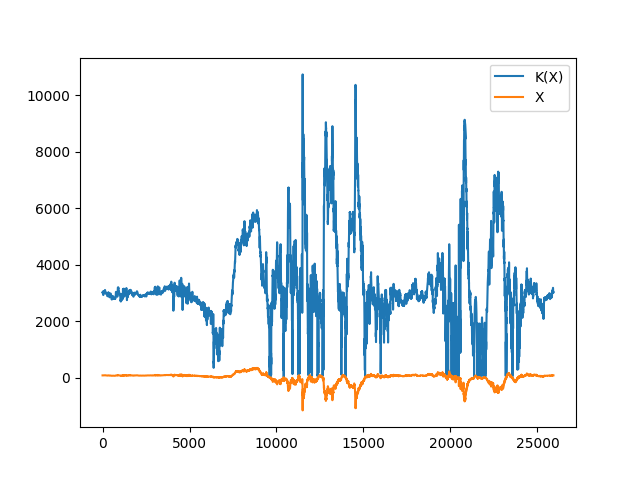
\includegraphics[width=\columnwidth]{Latex/fsim.png}
	       \caption{Sensor data and transfer function data from Fort Simpson dataset}
	   \end{center}
	
	\end{figure*}  
   
   The function K (not to be confused with the K in \ref{discretization}) is the complete implementation of the 5-layer Quebec model. 
   
   \section{Benchmark}
   To evaluate the accuracy of the computer implementation, it must be compared to the results from the original paper. Table 4 in \cite{8859181} shows the values calculated by the transfer function. This can be compared to the results calculated using the computer implementation. 
   

   
   	\begin{figure*}
		\begin{center}
		    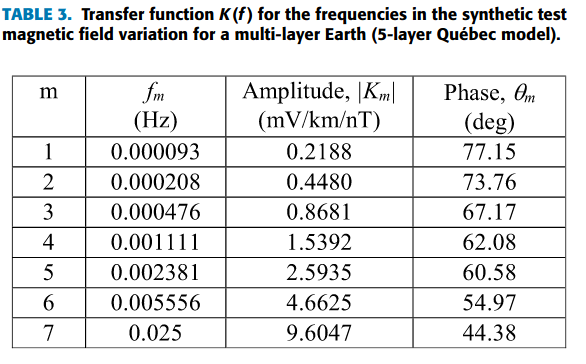
\includegraphics[width=\columnwidth]{Latex/Figure_3.png}
		    
		    %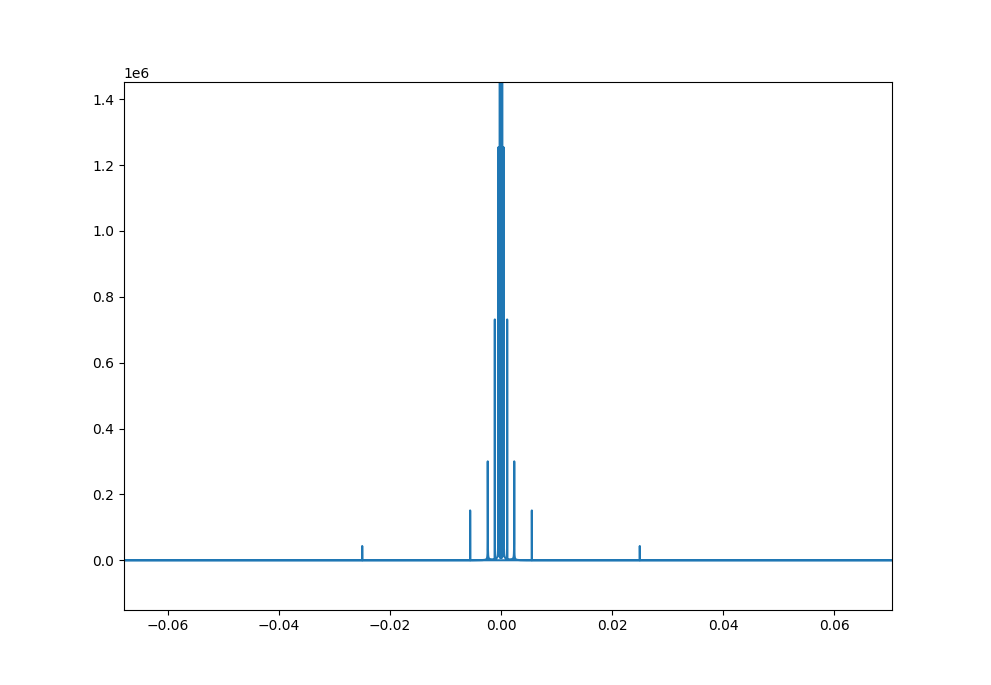
\includegraphics[width=\columnwidth]{Latex/Figure_2.png}
		        {\begin{tabular}{|c|c|c|c|}
        \hline
        
        \headcell{m}
        & \headcell{f_m}
        & \headcell{Amplitude}
        & \headcell{Phase} \\
        \hline
        1 & 0.000093 & 0.219701 & 77.139393 &
        \hline
        2 & 0.000208 & 0.447422 & 73.771382 &
        \hline
        3 & 0.000476 & 0.867800 & 67.172638 &
        \hline
        4 & 0.001111 & 1.539096 & 62.080986 &
        \hline
        5 & 0.002381 & 2.593561 & 60.575656 &
        \hline
        6 & 0.005556 & 4.662704 & 54.969143 &
        \hline
        7 & 0.025 & 9.604690 & 44.381495 &
        \hline
    \end{tabular}}
		    
		\end{center}

		\caption{Transfer function results from \cite{8859181}}
		\caption{Results from function implemented above}
	\end{figure*}
	
	Based on the tables, the computer simulation is very accurate; any inaccuracy is most likely due to the inaccuracy of calculations, constants, or the FFTW library. 
	
	\section{Real World Application}
	The 5 layer model implemented above can be used with real data rather than a simulated dataset. In this paper, a Fort Simpson, Canada dataset is used. For each value in the time-series data, the value was used as input to the transfer function \verb|K|. This can be vectorized in Julia like so:
	
	\begin{lstlisting}
Y = K.(X)
	\end{lstlisting}
	
	The lines below show both the input from the Fort Simpson data as well as the transfer function data.
	
    \section{Conclusion}
    This project develops a computer-based implementation of [CITATION]. Some challenges faced in this project were related to the nature of a computer-based implementation. For example, discretization was needed due to computer limitations. Additionally, speed was not a concern during the development. Because of this, the Julia programming language was often a bottleneck due to the Just In Time (JIT) compilation method. This makes Julia great for long running programs but often too slow for quick scripts. If reimplemented, a new implemention might include a compiled programming language like C or C++ for a faster runtime. Additionally, if further researched, a GIC solver would be created to determine the actual voltages and currents of the system that would be required.
	
	
\end{multicols}

\newpage
\newpage


\nocite{*}
\printbibliography
\small


%-----------------------------------------------------------------------------%


\end{document}
